\section{Preliminary Results}\label{sec:results}

\subsection{Model Building}

We build models as described in \secref{sec:training}. A few different model
types are shown in \figref{fig:models}.

\begin{figure*}
  \centering
  \begin{subfigure}[]{0.3\linewidth}
    \centering
    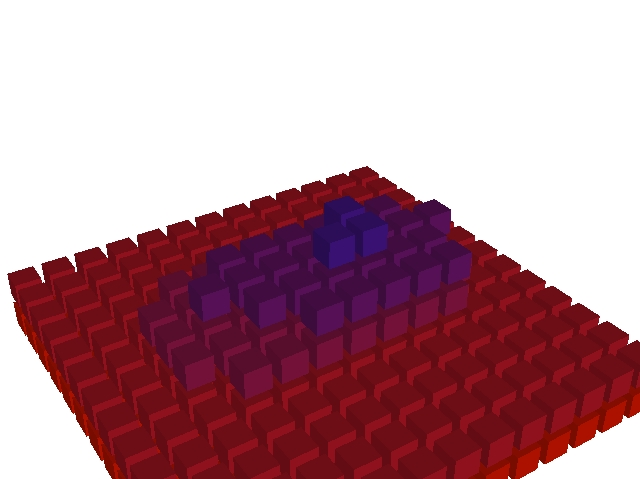
\includegraphics[height=1.5in]{figures/car_marginal.jpg}
    \caption{Na\"ive Bayes (\unit{50}{\cm})}
    \label{fig:nb}
  \end{subfigure}
  \begin{subfigure}[]{0.3\linewidth}
    \centering
    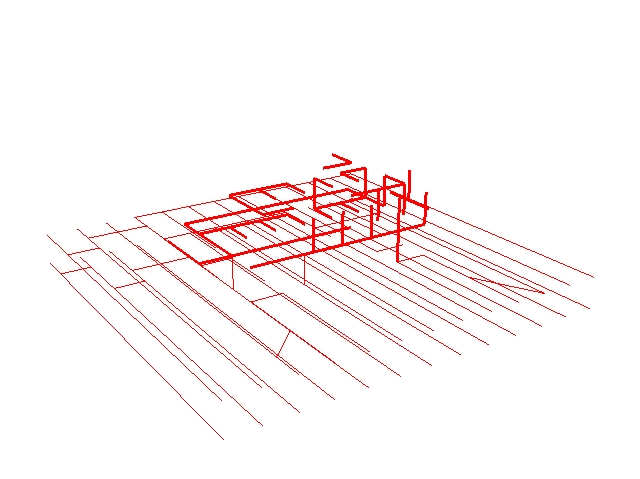
\includegraphics[height=1.5in]{figures/car_tree.jpg}
    %\caption{An example of a \ac{CLT} built for a car. For easier viewing, edges
    %  in the tree that link to nodes that are usually unoccupied are not rendered,
    %  and edges above the ground plane are rendered as thicker lines.}
    \caption{\ac{CLT} (\unit{50}{\cm})}
    \label{fig:clt}
  \end{subfigure}
  \begin{subfigure}[]{0.3\linewidth}
    \centering
    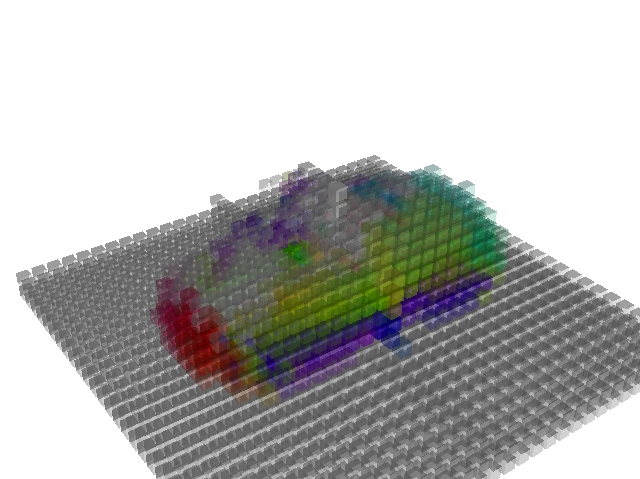
\includegraphics[height=1.5in]{figures/car_fm.jpg}
    \caption{Surface Normals (\unit{20}{\cm})}
    \label{fig:sn}
    %\caption{An example of a model with surface normals. Each voxel is colored by
    %  the most commonly observed surface normal orientation. The hue represents the
    %  surface normal's rotation about the vertical axis, and the saturation
    %  represents the surface normal's angle from the xy plane.}
  \end{subfigure}
  \caption{In \figref{fig:nb}, we see an example of a Na\"ive Bayes model for a
    car. Voxels are colored by z-height, and only voxels that are likely to be
    occupied are rendered. In \figref{fig:clt}, we see the \ac{CLT} as computed
    over the model. Only edges between voxels that are usually occupied are
    shown, with edges above the ground plane rendered as thicker lines. In
    \figref{fig:sn}, we see the model augmented with surface normals. Each voxel
    is colored by the most commonly observed surface normal orientation. The hue
    represents the surface normal's rotation about the vertical axis, and the
    saturation represents the surface normal's angle from the xy plane.}
  \label{fig:models}
\end{figure*}

\subsection{Detection Results}

While demonstrating some promising results (such as those shown in
\figref{fig:badge}, the proposed method still reports a significant number
of false positives. For example, in \figref{fig:ex2} the algorithm is able to
detect the two cars. However, it also believes that the building wall is a car,
due to the fact that it exhibits very similar structural appearance and surface
normals as the side of a car would. In \figref{fig:ex3}, we can see many correct
car detections on the road, but a similar problem occurs with the structure to
either side of the road. These examples were run using the model described in
\secref{sec:normals}, but similar behavior is exhibited with all models
described above.

\begin{figure}[!t]
  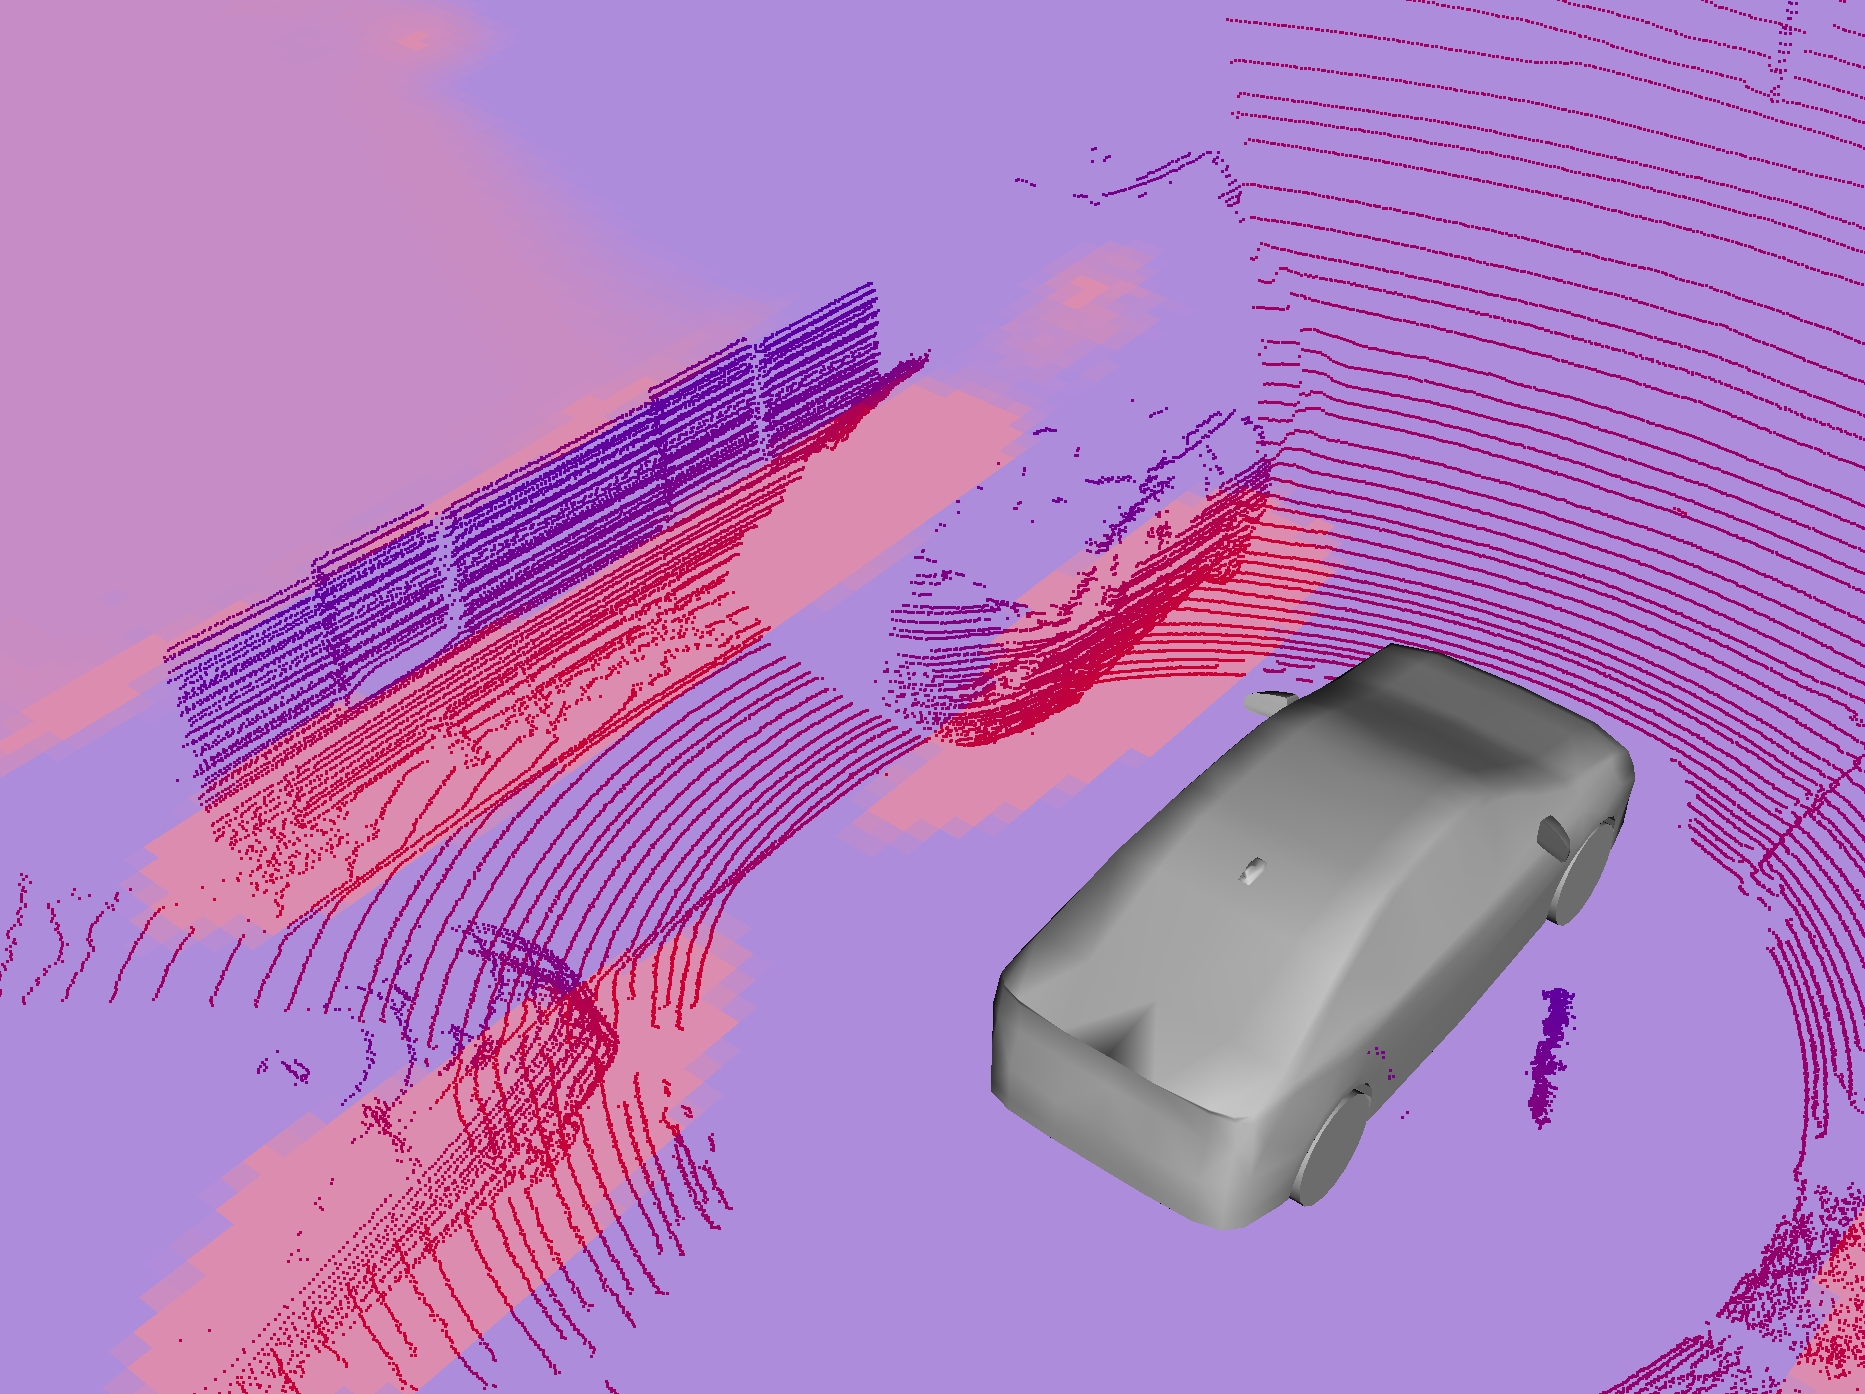
\includegraphics[width=\columnwidth]{figures/ex2.jpg}
  \caption{A very common fault case. Even with surface normals or a joint
    dependency model, often background such as building walls are supported by
    the car's  observation model. Car likelihoods are shown in red.}
  \label{fig:ex2}
\end{figure}

\begin{figure}[!t]
  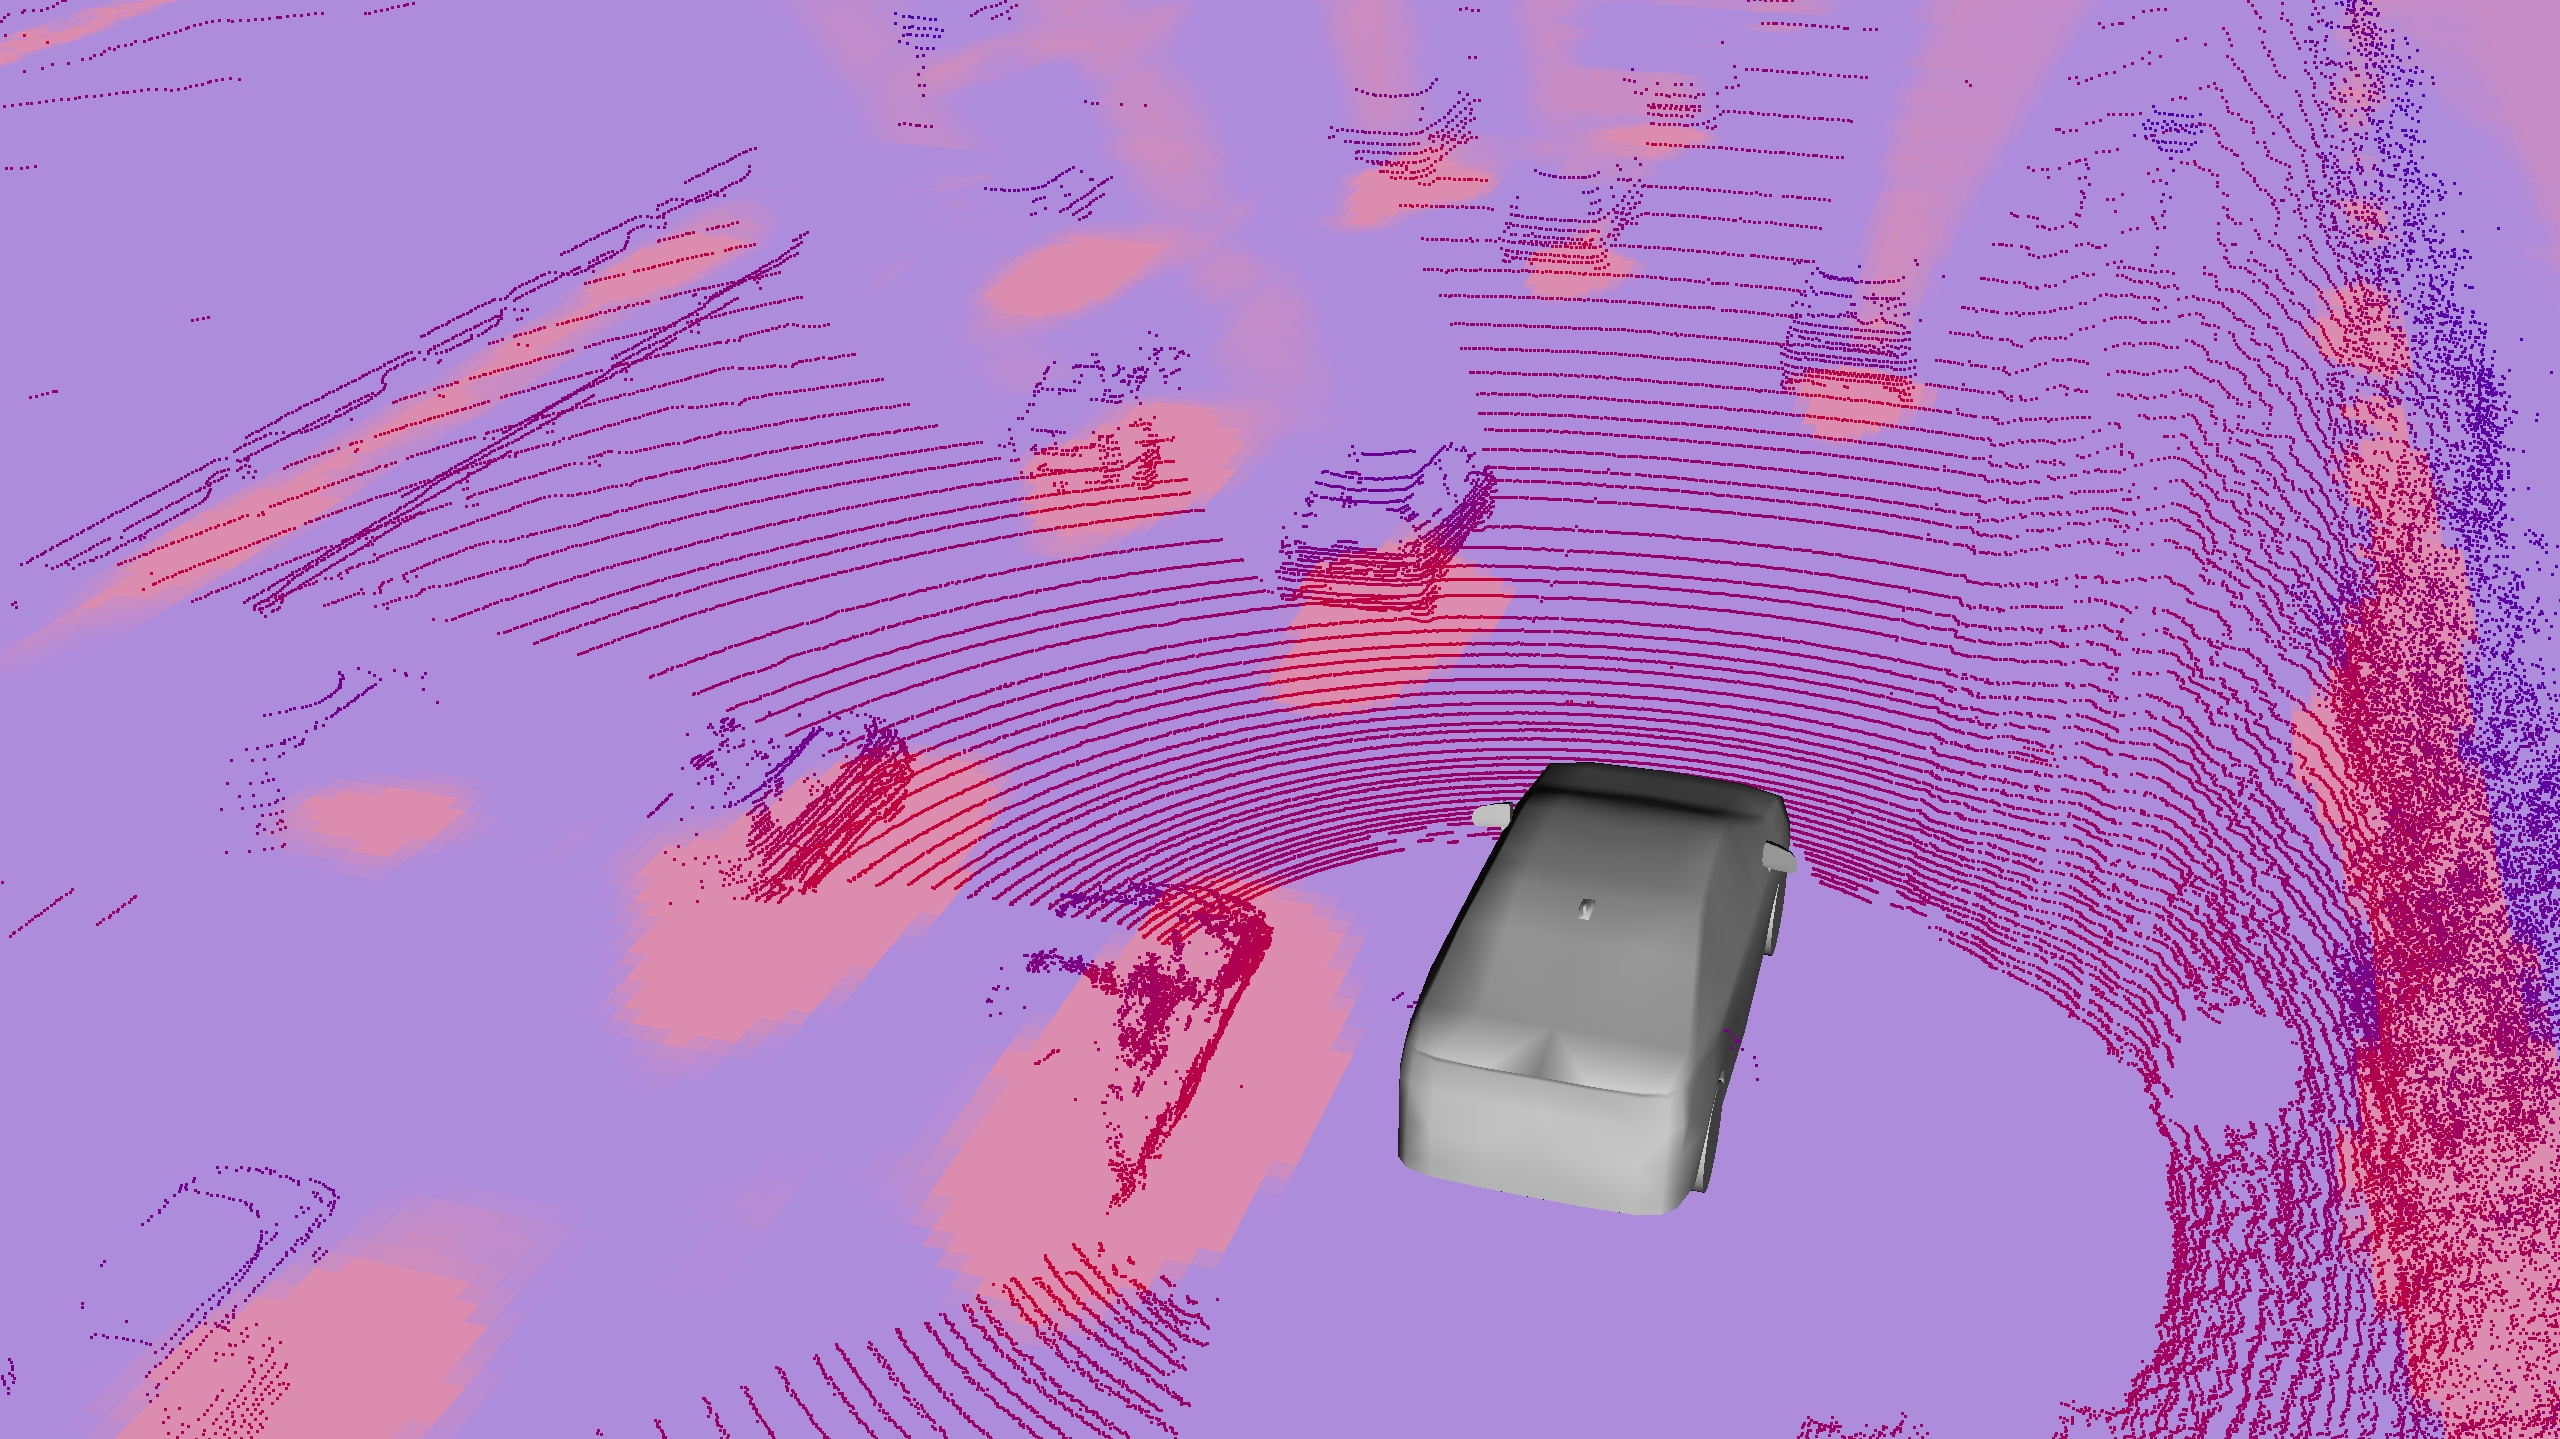
\includegraphics[width=\columnwidth]{figures/ex3.jpg}
  \caption{An example with both good detections and false positives on the
    background structure on either side of the road. Car likelihoods are shown
    in red.}
  \label{fig:ex3}
\end{figure}
